\chapter{Usporedba API-ja i ograničenja sustava}

\section{Usporedba aplikacijskih sučelja}

Za analizu razvojnog sustava korištena je mobilna aplikacija \textit{nRF Connect} tvrtke \textit{Nordic Semiconductor}. Pomoću nje moguće je pretražiti i povezati se sa BLE uređajima, kao i komunicirati s njima. Aplikacijom se također mogu analizirati podaci koje uređaj šalje pri oglašavanju te čitati informacije o samim uređajima i uslugama koje nude. \cite{nrfapp}

Jedna od mogućnosti aplikacije je i prikaz RSSI (engl. \textit{Received Signal Strength Indicator}) grafa. To je pokazatelj jačine primljenog signala te služi za mjerenje snage u primljenom radio signalu. RSSI je glavni indikator o jačini signala u danoj točki prostora. RSSI je relativna mjera, stoga je na grafičkom prikazu os RSSI vrijednosti označena dBm skalom, koja je negativna. 

Na slici \ref{fig:graph_comps} prikazan je RSSI graf za \textit{Bluedroid} demo aplikaciju \textit{BLE\_COMP\_TEST} učitanu na tri razvojna sustava. Mjerenje je obavljeno s udaljenosti od jednog metra, a sustavi su bili postavljeni u neposrednoj bliziini. Očitana srednja RSSI vrijednost je otprilike -50 dBm te je vidljiva pravokutna struktura signala. Na temelju RSSI skale \cite{rssi}, dobivena vrijednost označava jako dobru jačinu signala. Budući da RSSI vrijednosti uvelike variraju između proizvođača i modela proizvoda, te ovise o mobilnom uređaju koji ih mjeri, dobivene su drukčije vrijednosti za razvojne sustave s istim softverom. Iako graf nije indikator valjanosti softvera niti razvojnog sustava, zanimljivo je prikazati kako izmjerene vrijednosti dobivene s čipova istog proizvođača iz iste linije rezultiraju različitim vrijednostima.

Iduće je mjerenje obavljeno na jednom razvojnom sustavu, također s demo aplikacijom \textit{BLE\_COMP\_TEST}, te je svake sekunde jednakom količinom povećavana udaljenost mobilnog uređaja od razvojnog sustava radi prikazivanja ovisnosti RSSI vrijednosti o udaljenosti. Graf dobiven ovim mjerenjem prikazan je na slici \ref{fig:graph_distance}. Mjerenje je započeto na udaljenosti od nekoliko centimetara, što na grafu odgovara vrijednosti od -35 dBm, te završeno na udaljenosti od devet metara. Za konačnu udaljenost dobivena je vrijednost od otprilike -65 dBm, što je prema RSSI skali \cite{rssi} minimalna jačina za aplikacije koje zahtijevaju pouzdanu i pravovremenu isporuku podatkovnih paketa. Za ovisnost RSSI vrijednosti o udaljenosti dobivena je obrnuta proporcionalnost, što je u skladu sa zakonom inverznog kvadrata, koji tvrdi da je određena fizikalna veličina obrnuto proporcionalna kvadratu udaljenosti od izvora te fizikalne veličine.


\begin{figure}[ht]
	\begin{minipage}[t]{0.4\textwidth}
		\includegraphics[width=\linewidth]{imgs/graph\_comps}
		\caption{Graf RSSI vrijednosti za tri razvojna sustava}
		\label{fig:graph_comps}
	\end{minipage}
	\hspace*{\fill}
	\begin{minipage}[t]{0.4\textwidth}
		\includegraphics[width=\linewidth]{imgs/graph\_distance}
		\caption{Graf RSSI vrijednosti u ovisnosti o udaljenosti}
		\label{fig:graph_distance}
	\end{minipage}
\end{figure}


\section{Ograničenja razvojnog sustava}

Klasična Bluetooth tehnologija razvijena je kao bežični standard, što je omogućilo razvoj bežičnih i prenosivih uređaja. \textit{Classic BT} tehnologija koristi se za \textit{streaming} aplikacije, poput prijenosa audiozapisa i datoteka. Radi na istim frekvencijama kao i BLE, no ima veći broj RF kanala. Klasični Bluetooth ima veću propusnost podataka, čak do 3 Mbps, dok BLE propušta maksimalno 0.27 Mbps. Također ima veću brzinu prijenosa podataka, do 3 Mbps, u usporedbi sa BLE protokolom čija brzina doseže najviše 1 Mbps. Za razliku od BLE protokola čija je glavna odlika niska potrošnja,  zbog brze i nepredvidive komunikacije te složenih postupaka povezivanja \textit{Classic BT} troši znatno više energije i time brže troši bateriju uređaja na kojem se nalazi. Latencija prijenosa je čak 16 puta veća nego u BLE uređajima. Isto tako, podržava samo \textit{peer-to-peer} topologiju, odnosno 1:1, što znači da se istovremeno mogu povezati samo dva uređaja. Detaljnije razlike između verzija Bluetooth protokola nalaze se na slici \ref{fig:blevsbt}. \cite{blevsbt}

\begin{figure}[ht]
	\centering
	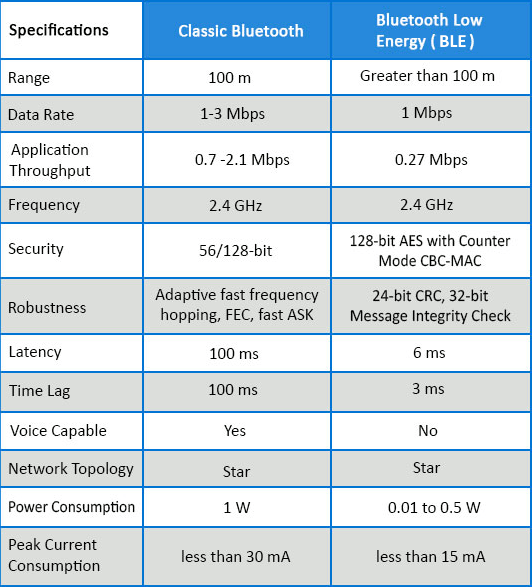
\includegraphics[scale=0.6]{imgs/blevsbt}
	\caption{Razlike između klasične Bluetooth i BLE tehnologije \cite{blevsbt}}
	\label{fig:blevsbt}
\end{figure}

Jedan nedostatak modula ESP32-C3 jest što ne podržava klasični Bluetooth. Iako BLE nudi prednosti u odnosu na \textit{Classic BT}, poput niske potrošnje i raznovrsnije podržane topologije, uređaji s BLE protokolom i s klasičnom Bluetooth tehnologijom ne mogu međusobno povezati. Ta činjenica ograničava povezivanje i korištenje ESP32-C3 modula, stoga ne može komunicirati s uređajima koji rade na temelju klasičnog Bluetootha. Većina audio uređaja, poput Bluetooth zvučnika, zbog potrebe za prijenosom velike količine podataka koriste klasični Bluetooth radi performansi. ESP32-C3 ne može se povezati s takvim uređajima.

Isto tako, BLE koristi pojas od 2,4 GHz kao i drugi bežični protokoli među kojima su Bluetooth i Wi-Fi. Zbog toga može doći do interferencije, što znači da dolazi do usporavanja prijenosa podataka među uređajima. Što se više uređaja nalazi na istoj frekvenciji, to su veća interferencija i latencija. Jedno od rješenja je fizički udaljiti uređaje koji koriste istu frekvenciju. \cite{limit_bt}

Kao što je ranije opisano, BLE uređaji mogu prenositi samo male količine podataka u kratkom vremenskom periodu.  Zbog tog ograničenja ne može primati izravne glasovne naredbe, što se često koristi u IoT uređajima. Ipak, postoje pomoćni uređaji koji pretvaraju zvučne signale u kratke nizove bajtova koji se zatim prosljeđuju uređaju. Jedan takav uređaj je tzv. \textit{voice assistant}.


\eject